\documentclass[dutch]{../khlslides}
\usepackage{graphicx}
\usepackage{pxfonts}
\usepackage{tikz}
\usepackage{calc}
\usepackage{fourier}

\usetikzlibrary{calc,shadows,decorations.markings}


\title{Introductie}
\logo{\includegraphics[height=0.5cm]{../KHL.jpg}}
\institute[KHL]{KHLeuven}

\newcommand{\AND}{\wedge}
\newcommand{\OR}{\vee}
\newcommand{\IMPLIES}{\rightarrow}
\newcommand{\IFF}{\leftrightarrow}
\newcommand{\NOT}{\neg}
\newcommand{\union}{\cup}
\newcommand{\intersect}{\cap}


\pgfkeys{
  /tikz/.cd,
  axis/.style={thin,-latex},
  plot/.style={domain=-5:5,thick}
}

\begin{document}

\maketitle

\begin{frame}
  \frametitle{Semesteroverzicht}
  \begin{center}
    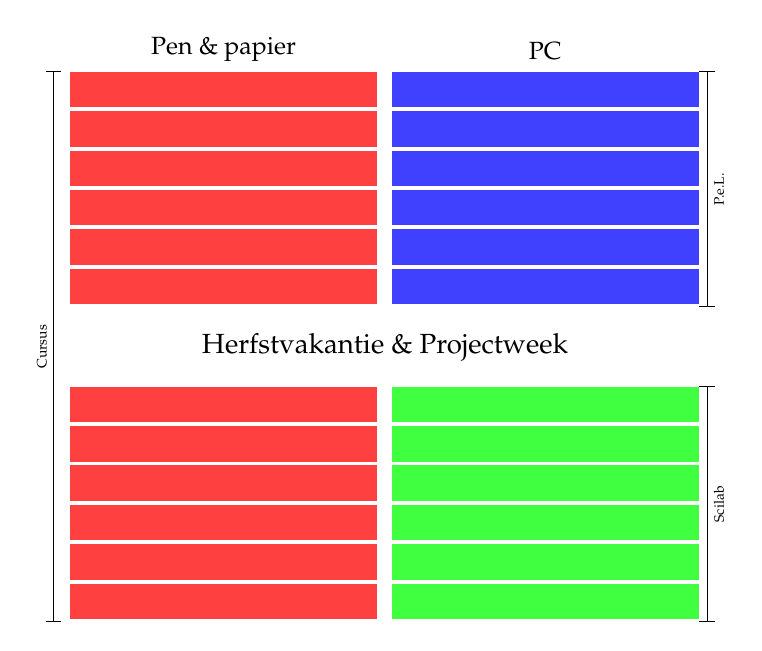
\begin{tikzpicture}
      \foreach \i in {1,...,6} {
        \pgfmathparse{\i * .5}\let\y\pgfmathresult
        \node[minimum width=3.9cm,minimum height=.45cm,fill=red!75,anchor=north west] at (0,\y) {};
      }

      \foreach \i in {7,...,12} {
        \pgfmathparse{\i * .5+1}\let\y\pgfmathresult
        \node[minimum width=3.9cm,minimum height=.45cm,fill=red!75,anchor=north west] at (0,\y) {};
      }

      \foreach \i in {1,...,6} {
        \pgfmathparse{\i * .5}\let\y\pgfmathresult
        \node[minimum width=3.9cm,minimum height=.45cm,fill=green!75,anchor=north east] at (8,\y) {};
      }

      \foreach \i in {7,...,12} {
        \pgfmathparse{\i * .5+1}\let\y\pgfmathresult
        \node[minimum width=3.9cm,minimum height=.45cm,fill=blue!75,anchor=north east] at (8,\y) {};
      }

      \draw[|-|] (-0.2,0) -- +(0,7) node [midway,sloped,yshift=1.5mm,font=\tiny] {Cursus};
      \draw[|-|] (8.1,4) -- +(0,3) node [midway,sloped,yshift=-1.5mm,font=\tiny] {P.e.L.};
      \draw[|-|] (8.1,0) -- +(0,3) node [midway,sloped,yshift=-1.5mm,font=\tiny] {Scilab};

      \node[anchor=north west,minimum size=8cm,minimum height=.8cm] at (0,3.9) {Herfstvakantie \& Projectweek};
      \node[anchor=south west,minimum size=3.9cm,minimum height=.5cm,font=\small] at (0,7) {Pen \& papier};
      \node[anchor=south east,minimum size=3.9cm,minimum height=.5cm,font=\small] at (8,7) {PC};
    \end{tikzpicture}
  \end{center}
\end{frame}

\begin{frame}
  \frametitle{Lessen}
  \begin{itemize}
    \item Twee keer per week
          \begin{itemize}
            \item E\'en uur in leslokaal
            \item E\'en uur in PC-lokaal
          \end{itemize}
    \item Geen aanwezigheden genomen
    \item Geen permanente evaluatie
    \item Geen toetsen of taken
    \item Enkel examen
  \end{itemize}
\end{frame}

\begin{frame}
  \frametitle{Examen}
  \begin{itemize}
    \item Combinatie schriftelijk en mondeling
    \item Toegelaten materiaal
          \begin{itemize}
            \item Formularium
            \item Rekenmachine
            \item PC (van de KHL)
          \end{itemize}
    \item Offici\"ele informatie: zie \href{http://onderwijsaanbod.khleuven.be/syllabi/n/MBI71AN.htm}{\beamergotobutton{ECTS}}
  \end{itemize}
\end{frame}

\end{document}



%%% Local Variables: 
%%% mode: latex
%%% TeX-master: t
%%% End: 
